\documentclass{standalone}
\usepackage{tikz}
\usetikzlibrary{patterns, positioning}
\usetikzlibrary{shapes.misc}
\usepackage[outline]{contour}
\contourlength{1.5pt} 
\usepackage[sfdefault]{ClearSans} %% option 'sfdefault' activates Clear Sans as the default text font
\usepackage[T1]{fontenc}

\begin{document}
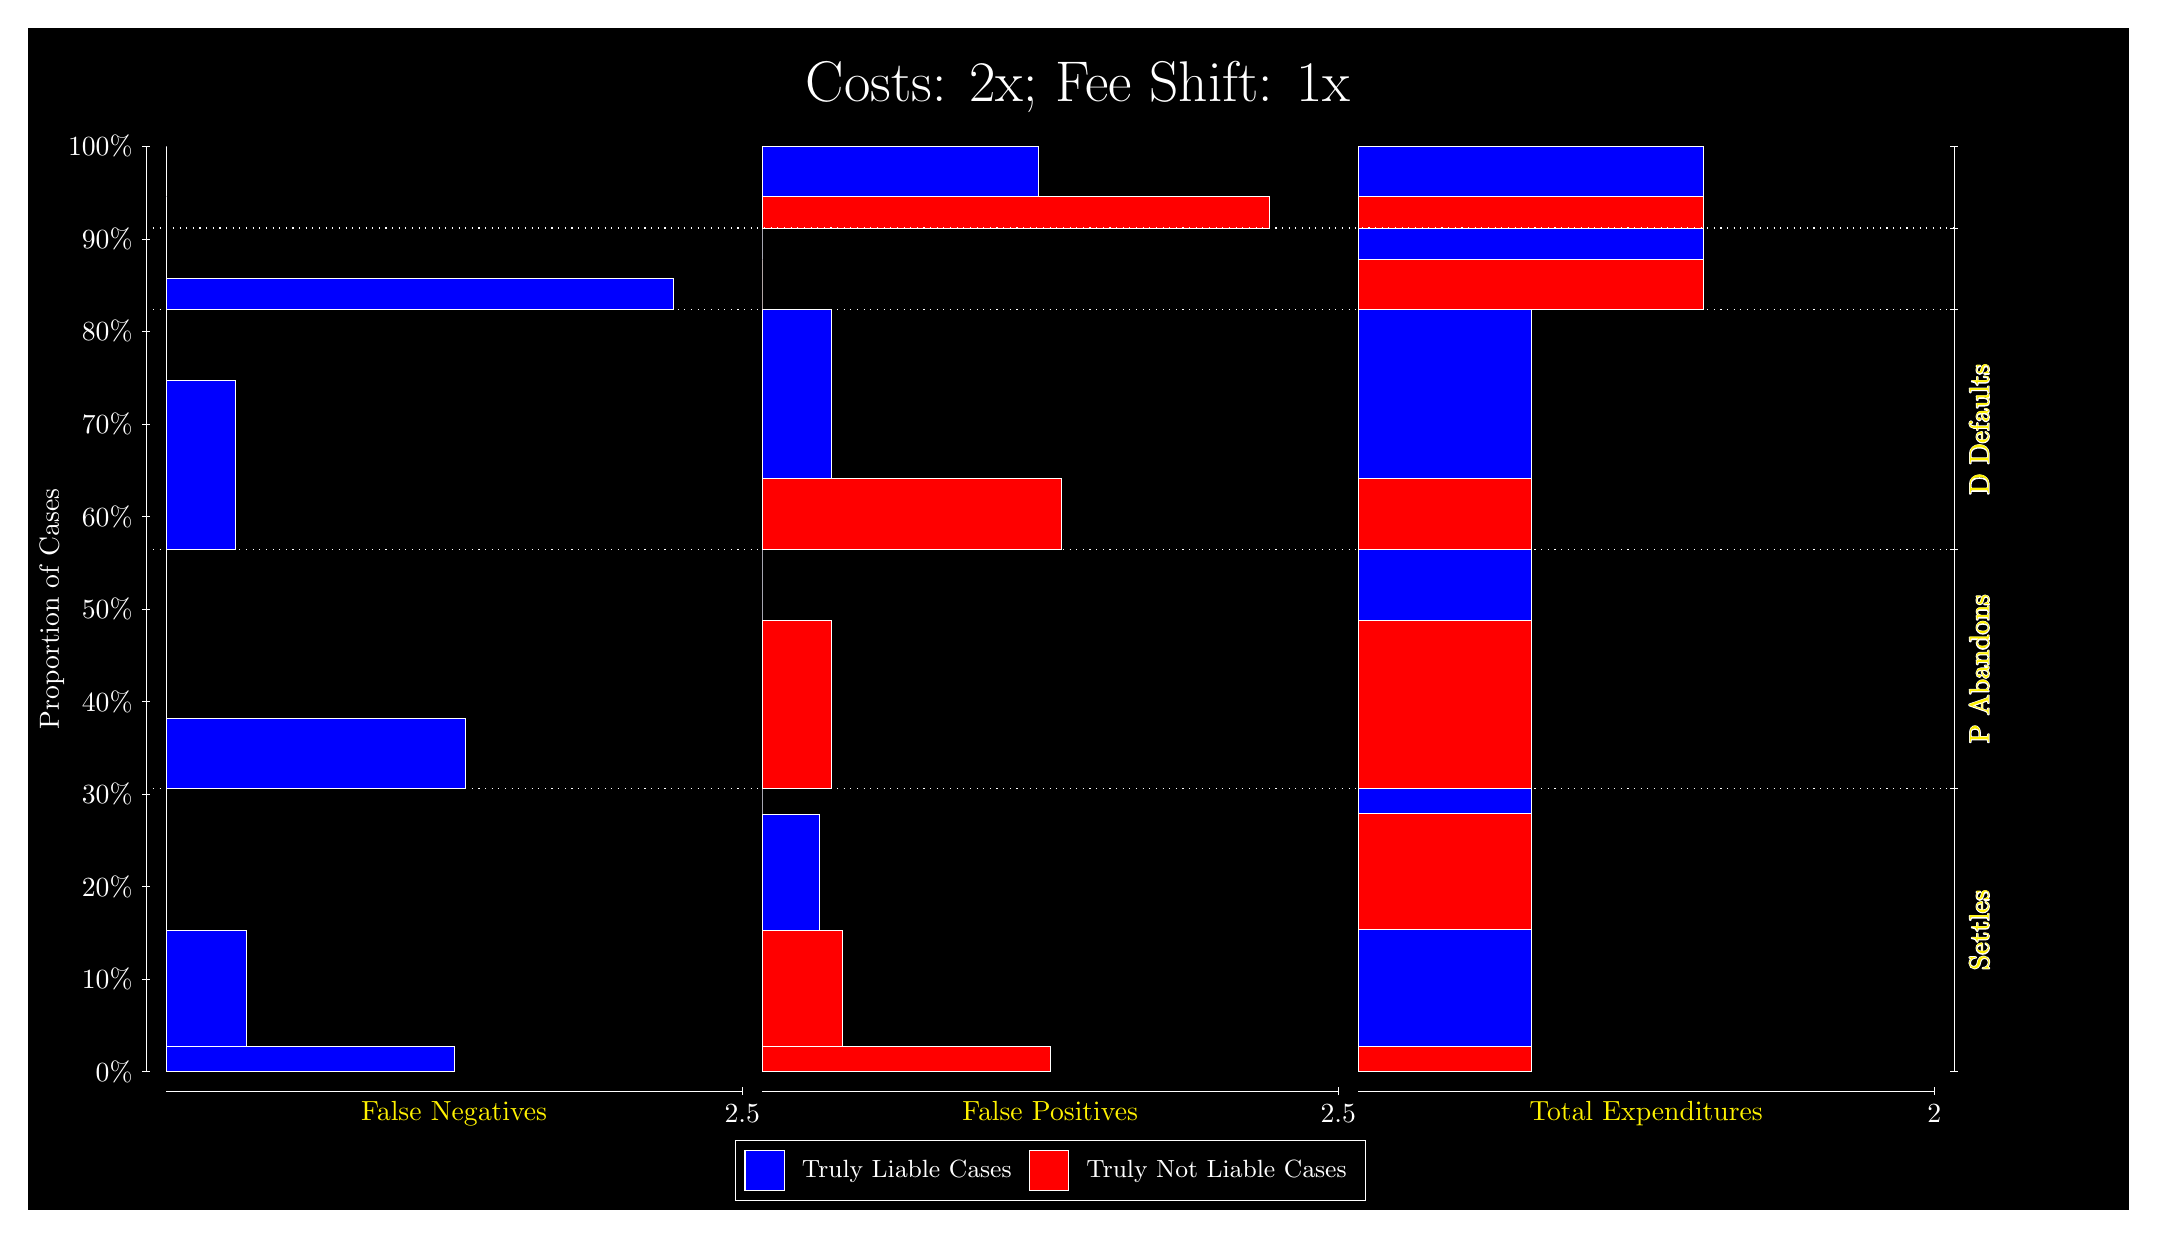
\begin{tikzpicture}
\draw[fill=black] (0,0) rectangle (26.667,15);
\draw[text=white] (0,13.5) rectangle (26.667,15) node[midway] {\huge Costs: 2x; Fee Shift: 1x};
\draw[white, very thin] (1.5,1.75) -- (1.5,13.5);
\node[rotate=90, text=white, anchor=center] at (0.3, 7.625) {Proportion of Cases};
\draw[white, very thin] (1.45,1.75) -- (1.55,1.75);
\node[text=white, anchor=east] at (1.45, 1.75) {0\%};
\draw[white, very thin] (1.45,2.925) -- (1.55,2.925);
\node[text=white, anchor=east] at (1.45, 2.925) {10\%};
\draw[white, very thin] (1.45,4.1) -- (1.55,4.1);
\node[text=white, anchor=east] at (1.45, 4.1) {20\%};
\draw[white, very thin] (1.45,5.275) -- (1.55,5.275);
\node[text=white, anchor=east] at (1.45, 5.275) {30\%};
\draw[white, very thin] (1.45,6.45) -- (1.55,6.45);
\node[text=white, anchor=east] at (1.45, 6.45) {40\%};
\draw[white, very thin] (1.45,7.625) -- (1.55,7.625);
\node[text=white, anchor=east] at (1.45, 7.625) {50\%};
\draw[white, very thin] (1.45,8.8) -- (1.55,8.8);
\node[text=white, anchor=east] at (1.45, 8.8) {60\%};
\draw[white, very thin] (1.45,9.975) -- (1.55,9.975);
\node[text=white, anchor=east] at (1.45, 9.975) {70\%};
\draw[white, very thin] (1.45,11.15) -- (1.55,11.15);
\node[text=white, anchor=east] at (1.45, 11.15) {80\%};
\draw[white, very thin] (1.45,12.325) -- (1.55,12.325);
\node[text=white, anchor=east] at (1.45, 12.325) {90\%};
\draw[white, very thin] (1.45,13.5) -- (1.55,13.5);
\node[text=white, anchor=east] at (1.45, 13.5) {100\%};

\draw[white, very thin] (24.457,1.75) -- (24.457,13.5);
\draw[white, very thin] (24.407,1.75) -- (24.507,1.75);
\node[anchor=west] at (24.407, 1.75) {};
\draw[white, very thin] (24.407,5.3429) -- (24.507,5.3429);
\node[anchor=west] at (24.407, 5.3429) {};
\draw[white, very thin] (24.407,8.3839) -- (24.507,8.3839);
\node[anchor=west] at (24.407, 8.3839) {};
\draw[white, very thin] (24.407,11.425) -- (24.507,11.425);
\node[anchor=west] at (24.407, 11.425) {};
\draw[white, very thin] (24.407,12.463) -- (24.507,12.463);
\node[anchor=west] at (24.407, 12.463) {};
\draw[white, very thin] (24.407,13.5) -- (24.507,13.5);
\node[anchor=west] at (24.407, 13.5) {};

\draw[white, very thin, fill=blue] (1.75,1.75) rectangle (5.4094,2.0675);
\draw[white, very thin, fill=blue] (1.75,2.0675) rectangle (4.092,2.0734);
\draw[white, very thin, fill=blue] (1.75,2.0734) rectangle (2.7746,3.5463);
\draw[white, very thin, fill=red] (1.75,3.5463) rectangle (1.75,5.3429);
\draw[white, very thin, fill=blue] (1.75,5.3429) rectangle (5.5558,6.2399);
\draw[white, very thin, fill=red] (1.75,6.2399) rectangle (1.75,8.3839);
\draw[white, very thin, fill=blue] (1.75,8.3839) rectangle (2.6283,10.528);
\draw[white, very thin, fill=red] (1.75,10.528) rectangle (1.75,11.425);
\draw[white, very thin, fill=blue] (1.75,11.425) rectangle (8.1906,11.827);
\draw[white, very thin, fill=red] (1.75,11.827) rectangle (1.75,12.463);
\draw[white, very thin, fill=red] (1.75,12.463) rectangle (1.75,12.865);
\draw[white, very thin, fill=blue] (1.75,12.865) rectangle (1.75,13.5);
\draw[white, very thin, fill=red] (9.3189,1.75) rectangle (12.978,2.0674);
\draw[white, very thin, fill=red] (9.3189,2.0674) rectangle (11.661,2.0733);
\draw[white, very thin, fill=red] (9.3189,2.0733) rectangle (10.344,3.5466);
\draw[white, very thin, fill=blue] (9.3189,3.5466) rectangle (10.051,5.0195);
\draw[white, very thin, fill=blue] (9.3189,5.0195) rectangle (9.3189,5.3429);
\draw[white, very thin, fill=red] (9.3189,5.3429) rectangle (10.197,7.4869);
\draw[white, very thin, fill=blue] (9.3189,7.4869) rectangle (9.3189,8.3839);
\draw[white, very thin, fill=red] (9.3189,8.3839) rectangle (13.125,9.2811);
\draw[white, very thin, fill=blue] (9.3189,9.2811) rectangle (10.197,11.425);
\draw[white, very thin, fill=red] (9.3189,11.425) rectangle (9.3189,12.061);
\draw[white, very thin, fill=blue] (9.3189,12.061) rectangle (9.3189,12.463);
\draw[white, very thin, fill=red] (9.3189,12.463) rectangle (15.759,12.865);
\draw[white, very thin, fill=blue] (9.3189,12.865) rectangle (12.832,13.5);
\draw[white, very thin, fill=red] (16.888,1.75) rectangle (19.083,2.0733);
\draw[white, very thin, fill=blue] (16.888,2.0733) rectangle (19.083,3.552);
\draw[white, very thin, fill=red] (16.888,3.552) rectangle (19.083,5.0254);
\draw[white, very thin, fill=blue] (16.888,5.0254) rectangle (19.083,5.3429);
\draw[white, very thin, fill=red] (16.888,5.3429) rectangle (19.083,7.4869);
\draw[white, very thin, fill=blue] (16.888,7.4869) rectangle (19.083,8.3839);
\draw[white, very thin, fill=red] (16.888,8.3839) rectangle (19.083,9.2811);
\draw[white, very thin, fill=blue] (16.888,9.2811) rectangle (19.083,11.425);
\draw[white, very thin, fill=red] (16.888,11.425) rectangle (21.279,12.061);
\draw[white, very thin, fill=blue] (16.888,12.061) rectangle (21.279,12.463);
\draw[white, very thin, fill=red] (16.888,12.463) rectangle (21.279,12.865);
\draw[white, very thin, fill=blue] (16.888,12.865) rectangle (21.279,13.5);
\draw[white, dotted] (1.5,5.3429) -- (24.457,5.3429);
\draw[white, dotted] (1.5,8.3839) -- (24.457,8.3839);
\draw[white, dotted] (1.5,11.425) -- (24.457,11.425);
\draw[white, dotted] (1.5,12.463) -- (24.457,12.463);
\draw[white, very thin] (1.75,1.5) -- (9.0689,1.5);
\node[text=yellow, anchor=north] at (5.4094, 1.5) {False Negatives};
\draw[white, very thin] (9.0689,1.45) -- (9.0689,1.55);
\node[text=white, anchor=north] at (9.0689, 1.45) {2.5};

\draw[white, very thin] (9.3189,1.5) -- (16.638,1.5);
\node[text=yellow, anchor=north] at (12.978, 1.5) {False Positives};
\draw[white, very thin] (16.638,1.45) -- (16.638,1.55);
\node[text=white, anchor=north] at (16.638, 1.45) {2.5};

\draw[white, very thin] (16.888,1.5) -- (24.207,1.5);
\node[text=yellow, anchor=north] at (20.547, 1.5) {Total Expenditures};
\draw[white, very thin] (24.207,1.45) -- (24.207,1.55);
\node[text=white, anchor=north] at (24.207, 1.45) {2};

\node[text=yellow, centered, rotate=90] at (24.777, 3.5464) {\contour{white}{Settles}};
\node[text=yellow, centered, rotate=90] at (24.777, 6.8634) {\contour{white}{P Abandons}};
\node[text=yellow, centered, rotate=90] at (24.777, 9.9046) {\contour{white}{D Defaults}};



\draw (12.978300999999998,1.5) node[draw=none] (baseCoordinate) {};
\begin{scope}[align=center]
        \matrix[scale=0.5, draw=white, below=0.5cm of baseCoordinate, nodes={draw}, column sep=0.1cm]{
            \node[rectangle, draw, minimum width=0.5cm, minimum height=0.5cm, fill=blue] {}; &
            \node[draw=none, font=\small, text=white] (B) {Truly Liable Cases}; &
            \node[rectangle, draw, minimum width=0.5cm, minimum height=0.5cm, fill=red] {}; &
            \node[draw=none, font=\small, text=white] (B) {Truly Not Liable Cases}; \\
            };
\end{scope}

\end{tikzpicture}
\end{document}